%%%%%%%%%%%%
%
% $Autor: Wings $
% $Datum: 2019-03-05 08:03:15Z $
% $Pfad: LoRaWan.tex $
% $Version: 4250 $
% !TeX spellcheck = en_GB/de_DE
% !TeX encoding = utf8
% !TeX root = filename 
% !TeX TXS-program:bibliography = txs:///biber
%
%%%%%%%%%%%%
\chapter{LoRaWan}


\begin{center}
    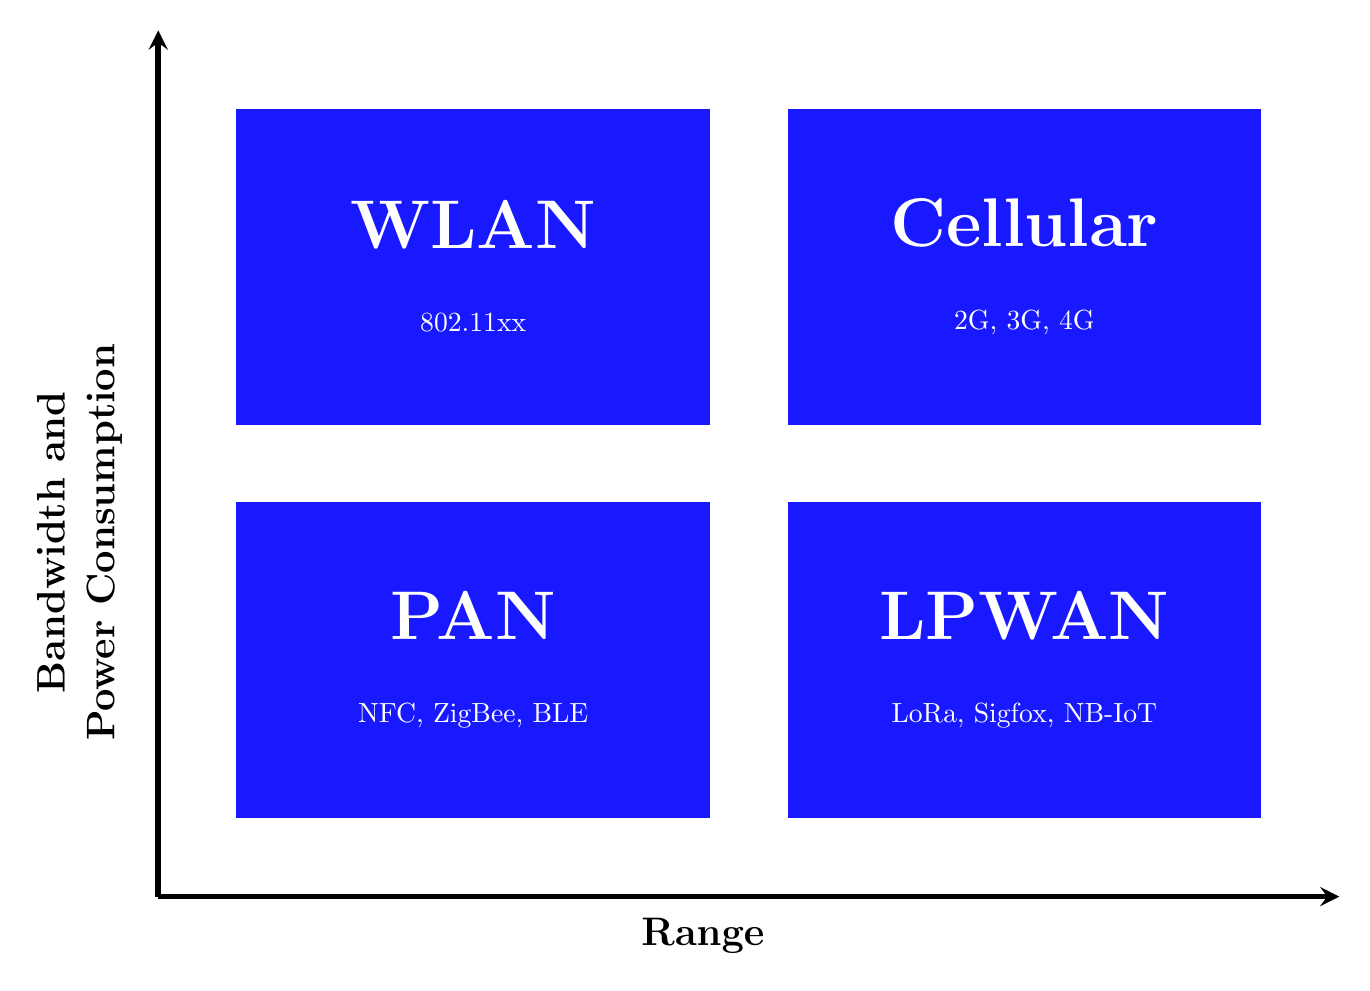
\begin{tikzpicture}
        % First Rectangle
        \draw[Blue!90, fill=Blue!90] (0,0) rectangle (6,4);
        \node[white, align=center, font=\Huge] at (3,2) {%
            \textbf{WLAN}
            \\
            \normalsize 802.11xx
        };
        
        % Second Rectangle
        \draw[Blue!90, fill=Blue!90] (7,0) rectangle (13,4);
        \node[white, align=center, font=\Huge] at (10,2) {%
            \textbf{Cellular}
            \\
            \normalsize 2G, 3G, 4G
        };
        
        % Third Rectangle
        \draw[Blue!90, fill=Blue!90] (0,-1) rectangle (6,-5);
        \node[white, align=center, font=\Huge] at (3, -3) {%
            \textbf{PAN}
            \\
            \normalsize NFC, ZigBee, BLE
        };
        
        % Fourth Rectangle
        \draw[Blue!90, fill=Blue!90] (7,-1) rectangle (13,-5);
        \node[white, align=center, font=\Huge] at (10,-3) {%
            \textbf{LPWAN}
            \\
            \normalsize LoRa, Sigfox, NB-IoT
        };
        
        % Horizontal arrow
        \draw[line width=2pt, -stealth, solid] (-1,-6) -- (14,-6);
        \node[black, align=center, font=\Large] at (6,-6.5) {%
            \textbf{Range}
        };
        
        % Vertical arrow
        \draw[line width=2pt, -stealth, solid] (-1,-6) -- (-1,5);
        \node[rotate=90, black, align=center, font=\Large] at (-2,-1.5) {%
            \textbf{Bandwidth and} \\
            \textbf{Power Consumption}
        };
    \end{tikzpicture}
\end{center}
